% Latex template: mahmoud.s.fahmy@students.kasralainy.edu.eg
% For more details: https://www.sharelatex.com/learn/Beamer

\documentclass{beamer}					% Document class

\usepackage[english]{babel}				% Set language
\usepackage[utf8x]{inputenc}			% Set encoding
\usepackage{tikz}
\usepackage{pgfplots}

\pgfplotsset{compat=1.18}
\mode<presentation>						% Set options
{
  \usetheme{default}					% Set theme
  \usecolortheme{default} 				% Set colors
  \usefonttheme{default}  				% Set font theme
  \setbeamertemplate{caption}[numbered]	% Set caption to be numbered
}

% Uncomment this to have the outline at the beginning of each section highlighted.
%\AtBeginSection[]
%{
%  \begin{frame}{Outline}
%    \tableofcontents[currentsection]
%  \end{frame}
%}

\usepackage{graphicx}					% For including figures
\usepackage{booktabs}					% For table rules
\usepackage{hyperref}					% For cross-referencing

\title{Predictive Analytics: Soccer Performance Data and All-SEC Honors}	% Presentation title
\author{Caleb Reid}								% Presentation author
\institute{University of Oklahoma}					% Author affiliation
\date{\today}									% Today's date	

\begin{document}

% Title page
% This page includes the informations defined earlier including title, author/s, affiliation/s and the date
\begin{frame}
  \titlepage
\end{frame}

% Outline
% This page includes the outline (Table of content) of the presentation. All sections and subsections will appear in the outline by default.
\begin{frame}{Outline}
\begin{columns}[c]

% Left column
\column{0.65\textwidth}

\tableofcontents

% Right column
\column{0.35\textwidth}

\centering
\includegraphics[width=\textwidth]{soccer-women.png}

\end{columns}
\end{frame}


% The following is the most frequently used slide types in beamer
% The slide structure is as follows:
%
%\begin{frame}{<slide-title>}
%	<content>
%\end{frame}
\begin{frame}[plain]

\centering

\vfill

{\Huge\bfseries Introduction}

\vfill

\end{frame}
\section{Introduction}

\begin{frame}{Introduction: SEC}
\begin{columns}[c]

% Left column
\column{0.65\textwidth}

	What is the SEC?
    \begin{itemize}
		\item Southeastern Conference (SEC): NCAA Division I Athletic Conference
        \item Consists of 16 teams including Oklahoma and Texas (since 2024)
	\end{itemize}

% Right column
\column{0.35\textwidth}

\centering
\includegraphics[width=\textwidth]{OIP.png}

\end{columns}
    
\end{frame}

\begin{frame}{Introduction: All-SEC}


    What does All-SEC mean?
    \begin{itemize}
		\item Recognizes the most outstanding women's soccer athletes during the SEC regular season including:
        \begin{itemize}
            \item First-Team All-SEC
            \item Second-Team All-SEC
            \item Third-Team All-SEC
        \end{itemize}
        \item Voted on by the league's 16 coaches
	\end{itemize}

\end{frame}

\begin{frame}{Introduction: Wyscout}

\begin{columns}[c]

% Left column
\column{0.35\textwidth}

Wyscout
\begin{itemize}
    \item The world’s biggest library of soccer video and data
    \begin{itemize}
        \item Purchased by Hudl in 2019
    \end{itemize}
    \item Provides performance data to every SEC team
    \begin{itemize}
        \item Team-level data
        \item Player-level data
    \end{itemize}
\end{itemize}

% Right column
\column{0.65\textwidth}

\centering
\includegraphics[width=\textwidth]{wyscoutExample.png}

\end{columns}


\end{frame}

\begin{frame}{Introduction: Research Question}

\begin{columns}[c]

\column{0.42\textwidth}
\centering
Does placing in the top 10 of SEC performance categories

\column{0.16\textwidth}
\centering
{\Huge $\rightarrow$}

\column{0.42\textwidth}
\centering
All-SEC honors?

\end{columns}

\end{frame}

\begin{frame}[plain]

\centering

\vfill

{\Huge\bfseries Data}

\vfill

\end{frame}

\section{Data}

\begin{frame}{Data}
	\input{tables/dataSources}
\end{frame}

\begin{frame}{Data}
\centering
\includegraphics[width=\textwidth]{dataOverviewTable.png}

\end{frame}

\begin{frame}{Data}
\centering
\includegraphics[width=\textwidth]{posBreakdown.png}

\end{frame}

\begin{frame}[plain]

\centering

\vfill

{\Huge\bfseries Methods}

\vfill

\end{frame}

\section{Methods}
\begin{frame}{Methods}
\[
\log\left(
\frac{P(\text{allSEC}=1)}
{1-P(\text{allSEC}=1)}
\right)
=
\beta_0
+
\sum_{j=1}^{13}\beta_jX_j
\]

{\footnotesize
\[
X_j =
\{
\text{year, pos, goalsPer90, assistsPer90, shotsPer90,}
\]
\[
\text{keyPassesPer90, touchesBoxPer90, defDuelsPer90,}
\]
\[
\text{aerialDuelsPer90, recoveriesPer90, interceptionsPer90,}
\]
\[
\text{slidingTacklesPer90, shotsBlockedPer90}
\}
\]
}
	Model:
    \begin{itemize}
		\item Elastic net logistic regression model
        \item Penalty tuned to mixture = 0.75
        \item Five-fold cross validation
        \begin{itemize}
            \item Tuned using Cohen's Kappa
            \item Stratified on allSEC
        \end{itemize}
	\end{itemize}
\end{frame}
\begin{frame}[plain]

\centering

\vfill

{\Huge\bfseries Results}

\vfill

\end{frame}

\section{Results}

\begin{frame}{Results}

\begin{center}
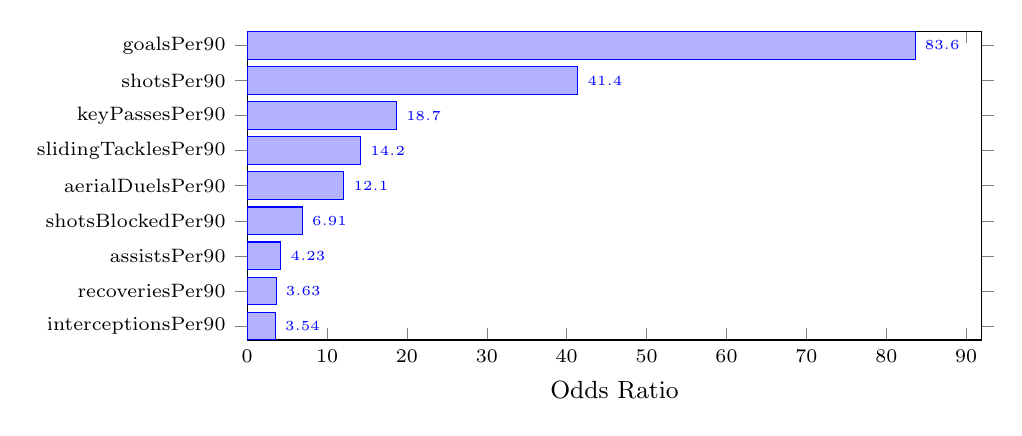
\begin{tikzpicture}
\begin{axis}[
    xbar,
    width=0.9\textwidth,
    height=5.5cm,
    xmin=0,
    xlabel={Odds Ratio},
    symbolic y coords={
        interceptionsPer90,
        recoveriesPer90,
        assistsPer90,
        shotsBlockedPer90,
        aerialDuelsPer90,
        slidingTacklesPer90,
        keyPassesPer90,
        shotsPer90,
        goalsPer90
    },
    ytick=data,
    nodes near coords,
    nodes near coords align={horizontal},
    enlarge y limits=0.05,
    tick label style={font=\scriptsize},
    label style={font=\small},
    every node near coord/.append style={
        font=\tiny
    }
]

\addplot coordinates {
    (83.6,goalsPer90)
    (41.4,shotsPer90)
    (18.7,keyPassesPer90)
    (14.2,slidingTacklesPer90)
    (12.1,aerialDuelsPer90)
    (6.91,shotsBlockedPer90)
    (4.23,assistsPer90)
    (3.63,recoveriesPer90)
    (3.54,interceptionsPer90)
};

\end{axis}
\end{tikzpicture}
\end{center}

\end{frame}

\begin{frame}{Results}
\begin{columns}
    \column{.35\textwidth}
Model performance:
    \begin{itemize}
		\item Kappa = 0.48
        \item Sensitivity = 0.44
	\end{itemize}

    \column{.65\textwidth}
    	\begin{figure}[H]
        \includegraphics[width=1.0\textwidth]{confusionMatrixGT2.png}
        \caption{Test data}
        \label{fig:figure1}
	\end{figure}
\end{columns}
\end{frame}

\begin{frame}[plain]

\centering

\vfill

{\Huge\bfseries Discussion}

\vfill

\end{frame}

\section{Discussion}

\begin{frame}{Discussion}
	Attacks reign supreme:
    \begin{itemize}
		\item Top three most influential features were attacking stats
        \item Being amongst the top 10 of goals (per 90 mins) increases your chance of being selected to an All-SEC team by 84\%!
	\end{itemize}

    	Model is not a great predictor of All-SEC awards:
    \begin{itemize}
		\item Missed three All-SEC players
        \item Misidentified four null players
	\end{itemize}
\end{frame}

\begin{frame}{Discussion}
	\begin{columns}
		\column{.5\textwidth}
        Limitations:
    \begin{itemize}
		\item Wyscout data only provided for players who finished in the top 10 of the respective category
        \item Wyscout data was in a .pdf form which could negatively impact the validity of the data
        \item Variables were chosen based on prior knowledge
        \item No unique identifiers for similar players
        \item Only generalizable to women's soccer All-SEC teams
	\end{itemize}
        
        \column{.5\textwidth}
        Future research:
    \begin{itemize}
		\item Include performance data for ALL athletes
        \item Cross-validate variables to increase validity and predictive power
        \item Increase sample size (number of years)
	\end{itemize}
	\end{columns}
\end{frame}
\begin{frame}[plain]

\centering

\vfill

{\Huge\bfseries Thank you!}

\vfill

\end{frame}

\end{document}
